\section{Cached evaluation}

\begin{frame}{Benchmark methodology}
We have conducted exhaustive benchmarks.\\
They are separated in three categories:

\begin{itemize}
	\item Comparison between cached over RADOS and RADOS solely
		\begin{itemize}
			\item Peak behavior
			\item Sustained behavior
		\end{itemize}
	\item Internal measurement of cached
		\begin{itemize}
			\item Indexing mechanism overhead
		\end{itemize}
	\item Evaluation of VM/Archipelago
\end{itemize}
\spc
Note: sosd refers to the blocker driver of Archipelago

\note{Οι μετρήσεις μας είναι εκτενείς και χωρίζονται σε τρεις κατηγορίες:
	\begin{itemize}
		\item Σύγκριση performance του cached και rados για workloads 
			μικρότερα και μεγαλύτερα του cache size
		\item Αξιολόγηση εσωτερικών κομματιών του cached (συγκεκριμένα overhead 
			του indexing μηχανισμού
		\item Μετρήσεις του Αρχιπελάγους για ένα πραγματικό VM
	\end{itemize}

	Στις επόμενες μετρήσεις, όπου sosd εννοούμε rados. Επίσης, όλα είναι random 
	i/o

	Σημείωση, τρίτη κατηγορία είναι πολύ σημαντική. Καταφέραμε να σηκώσουμε 
	πραγματικό VM με cached. Αυτό είναι το highlight της διπλωματικής
}

\end{frame}

\begin{frame}{Cached/sosd comparison - peak behavior}
	\begin{columns}[t]
		\begin{column}{.5\textwidth}
			Write bandwidth
			\makebox[\textwidth]{
				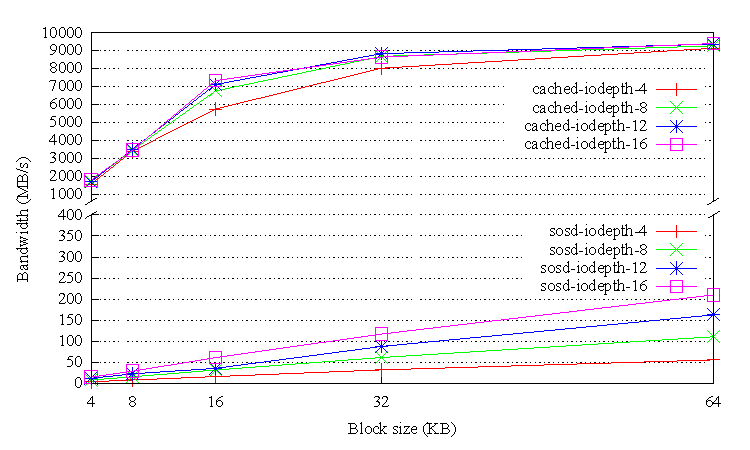
\includegraphics[width=\columnwidth]{images/bw-write-comp-lie.pdf}
			}
			Constants:
			\begin{itemize}
				\item cached has 4 threads
				\item workload size less than cache size
			\end{itemize}
		\end{column}
		\begin{column}{.5\textwidth}
			Read bandwidth
			\makebox[\textwidth]{
				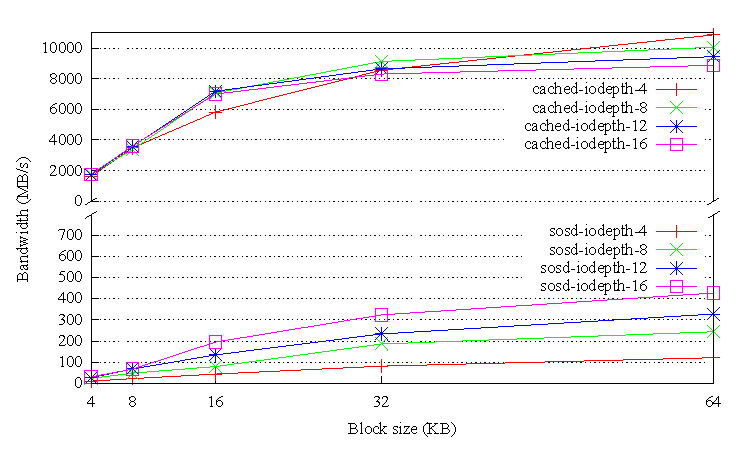
\includegraphics[width=\columnwidth]{images/bw-read-comp-lie.pdf}
			}
			Variables:
			\begin{itemize}
				\item block size [4KB - 64KB]
				\item parallel requests [4 - 16]
			\end{itemize}
		\end{column}
	\end{columns}

	\note[item]{Ας περιγράψουμε το benchmark μας. Στείλαμε καρφωτά στους peers 
		requests των...}
	\note[item]{Το iodepth είναι ο αριθμός των παράλληλων requests}
	\note[item]{Σημεία προσοχής:Για μικρά writes είμαστε έως 100x 
		γρηγορότεροι ενώ για μεγάλα έως 200x. }
	\note[item]{O cached μετά τα 16ΚΒ δεν κάνει scale - χτυπάμε το 
		bandwidth της RAM}
	\note[item]{Έχουμε lock contention, δε θα έπρεπε να αυξάνεται η 
		ταχύτητα για μεγάλα blocks και δεν αυξάνεται η ταχύτητα με 
		parallel requests}
	\note[item]{Lock contention είναι ότι δεν κάνουμε scale με πολλά threads 
		για μικρά block sizes}
\end{frame}

\begin{frame}{Cached/sosd comparison - peak behavior}
	\begin{columns}[t]
		\begin{column}{.5\textwidth}
			Write latency
			\makebox[\textwidth]{
				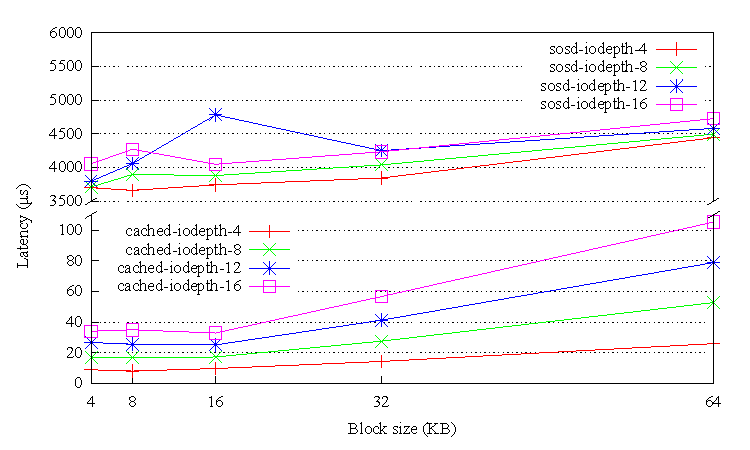
\includegraphics[width=\columnwidth]{images/lat-write-comp-lie.pdf}
			}
			Constants:
			\begin{itemize}
				\item cached has 4 threads
				\item workload size less than cache size
			\end{itemize}
		\end{column}
		\begin{column}{.5\textwidth}
			Read latency
			\makebox[\textwidth]{
				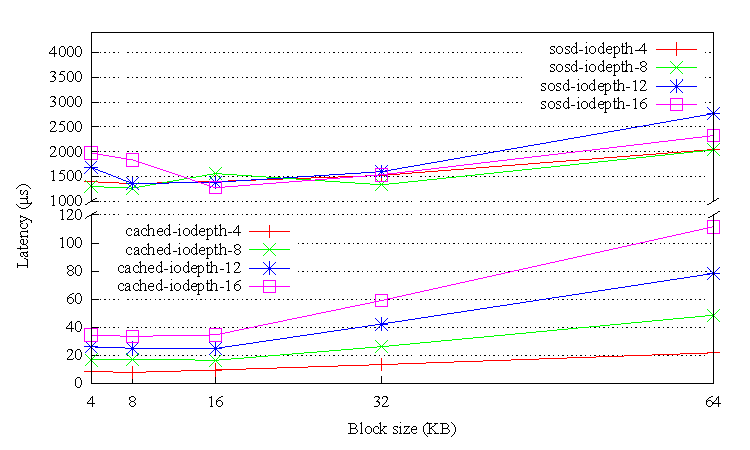
\includegraphics[width=\columnwidth]{images/lat-read-comp-lie.pdf}
			}
			Variables:
			\begin{itemize}
				\item block size [4KB - 64KB]
				\item parallel requests [4 - 16]
			\end{itemize}
		\end{column}
	\end{columns}

	\note[item]{Αντίστοιχα, για μικρά reads είμαστε 50x γρηγορότεροι ενώ 
		για μεγάλα έως 75x}
\end{frame}

\begin{frame}{Cached/sosd comparison - sustained behavior}
	\begin{columns}[t]
		\begin{column}{.5\textwidth}
			Write bandwidth
			\makebox[\textwidth]{
				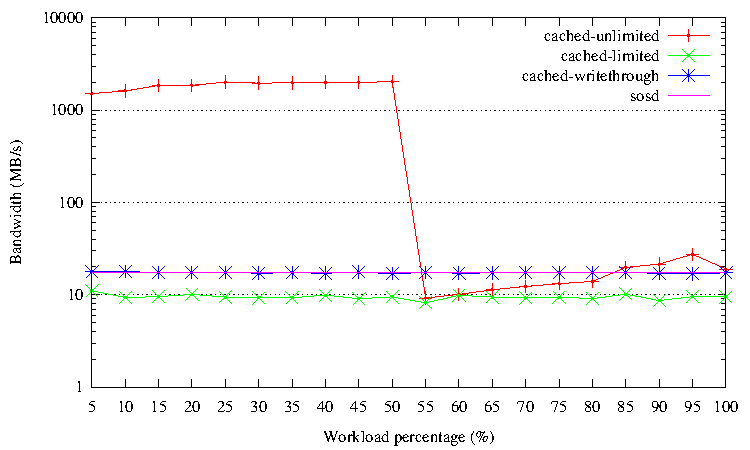
\includegraphics[width=\columnwidth]{images/bw-write-comp-truth.pdf}
			}
			Constants:
			\begin{itemize}
				\item cached has 4 threads
				\item workload twice the cache size
				\item block size is 4KB
				\item Parallel requests are 16
			\end{itemize}
		\end{column}
		\begin{column}{.5\textwidth}
			Write latency
			\makebox[\textwidth]{
				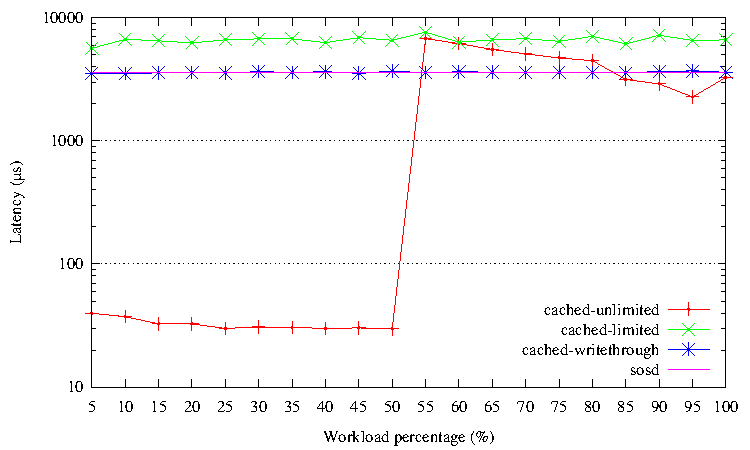
\includegraphics[width=\columnwidth]{images/lat-write-comp-truth.pdf}
			}
			Variables:
			\begin{itemize}
				\item cache write policy
				\item maximum cached objects
			\end{itemize}
		\end{column}
	\end{columns}

	\note[item]{unlimited: έχουμε περισσότερα buckets απ' ότι objects}
	\note[item]{Σημεία προσοχής: Writethrough όσο και το Rados ενώ στα 
		reads έχουμε παρατηρήσει καλύτερη ταχύτητα}
	\note[item]{Το performance πέφτει λόγω έλλειψης buckets, μεγαλώνει λόγω 
		coalesces}

\end{frame}

\begin{frame}{Cached internals - indexing}
	Latency of cold cache vs. warm cache
	\makebox[\textwidth]{
		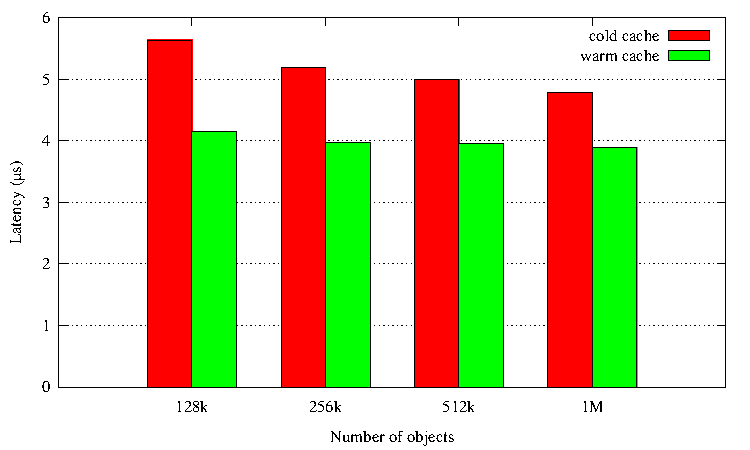
\includegraphics[width=0.45\textwidth]{images/cold1.pdf}
	}
	\begin{columns}[t]
		\begin{column}{.5\textwidth}
			Constants:
			\begin{itemize}
				\item workload less than the cache size
				\item block size is 4KB
				\item no threads or parallel requests 
			\end{itemize}
		\end{column}
		\begin{column}{.5\textwidth}
			Variables:
			\begin{itemize}
				\item number of objects [128k - 1M]
			\end{itemize}
		\end{column}
	\end{columns}
	\note[item]{Το σενάριο είναι το εξής. Εισάγουμε ένα αριθμό από objects.  
		Κάνουν lookup και insert. Μετά, τα κάνουμε lookup. Αυτό το κάνουμε για 
		128κ ... Μετράμε latency}
	\note[item]{Σταθερό indexing overhead. Αν πέσει ερώτηση πες 2Μ hash 
		table, το λειτουργικό δε δίνει αμέσως μνήμη}
\end{frame}

\begin{frame}{VM/Archipelago evaluation}
	\begin{columns}[t]
		\begin{column}{.5\textwidth}
			Write bandwidth
			\makebox[\textwidth]{
				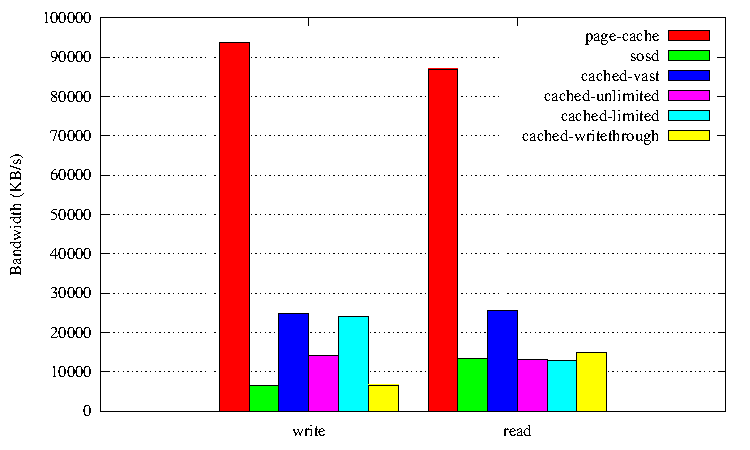
\includegraphics[width=\columnwidth]{images/bw-vm.pdf}
			}
			Constants:
			\begin{itemize}
				\item block size is 4KB
				\item parallel requests are 16
				\item cached has 4 threads
			\end{itemize}
		\end{column}
		\begin{column}{.5\textwidth}
			Write latency
			\makebox[\textwidth]{
				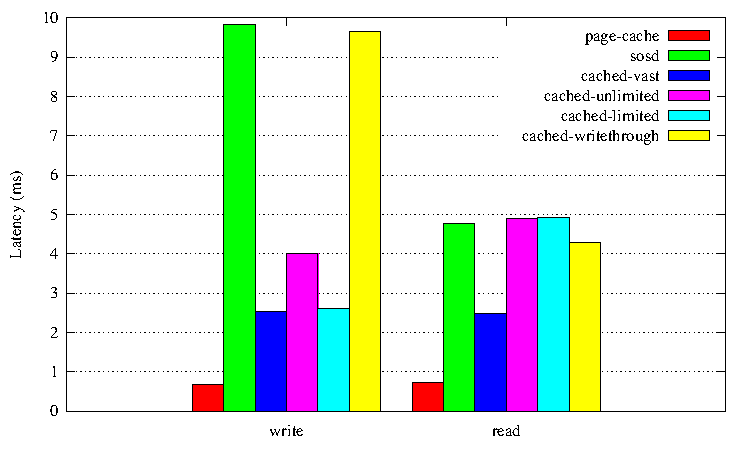
\includegraphics[width=\columnwidth]{images/lat-vm.pdf}
			}
			Variables:
			\begin{itemize}
				\item cache write policy
				\item maximum cached objects
			\end{itemize}
		\end{column}
	\end{columns}
	\note{Benchmark μέσα από το VM, με filesystem, elevators, κτλ. με το fio}
	\note{Σημεία προσοχής:
		\begin{itemize}
			\item page-cache: πολύ γρήγορη. Το 1ms latency λογικά 
				μπαίνει λόγω του paravirtualized storage, 
				filesystem, elevators
			\item sosd: είναι σίγουρα άσχημο αλλά σε αυτά τα test 
				έχει συν 7ms latency για τα writes και 3ms 
				latency για τα reads. Αυτό έιναι πολύ 
				μεγαλύτερο του 1ms του VM άρα κάτι παίζει με 
				Αρχιπέλαγο
			\item cached-vast: 4x γρηγορότερη από sosd αλλά έχει 
				3ms latency που δεν είχε πριν, δηλαδή το 
				archipelago βάζει 2ms
			\item cached-unlimited: 2.5x γρηγορότερο και ξεπέρασε 
				πάλι τον sosd στο τέλος
			\item cached-limited: 4x γρηγορότερο, λογικά τα flushes 
				είναι πολλα και μικρά και κρύβονται πίσω από το 
				latency του Archipelago
			\item writethrough δεν είδαμε κάποια διαφορά
		\end{itemize}
	}
\end{frame}




